\documentclass{article}
\usepackage{amsmath}
\usepackage{tikz}
\usetikzlibrary{arrows.meta, shapes.geometric, positioning}
\usepackage{verbatimbox}
\usepackage{geometry}
\geometry{a4paper, margin=1in}

\title{How an Interpreted Language Works}
\author{}
\date{}

\begin{document}

\maketitle

\begin{center}

\section{Introduction}
An interpreted language works by executing code directly from its human-readable source form, without the need to compile it into machine code beforehand. This document explains the components of an interpreter and the process of interpreting code.

\section{Components of an Interpreter}

\subsection{Lexical Analysis}
Lexical Analysis, or tokenization, is the process of converting a sequence of characters into a sequence of tokens.

\subsection{Parsing}
Parsing involves analyzing the tokens to form a grammatical structure, typically represented by an Abstract Syntax Tree (AST).

\subsection{Semantic Analysis}
Semantic Analysis checks for semantic errors and ensures the operations in the code make sense.

\subsection{Execution}
Execution involves traversing the AST and performing the operations defined by the source code.

\section{Flowchart of Interpretation Process}

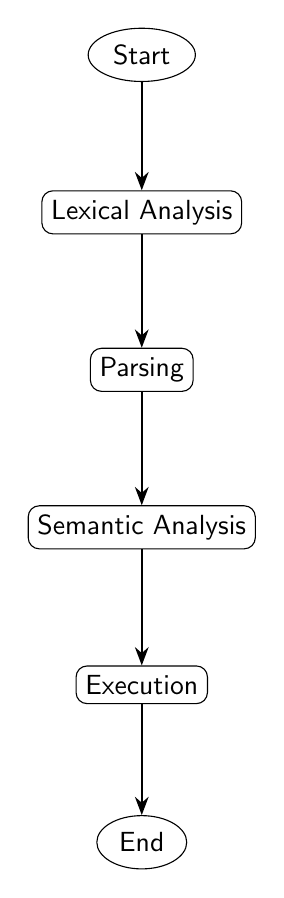
\begin{tikzpicture}[
  node distance=2cm, 
  every node/.style={rectangle, draw=black, rounded corners, align=center, font=\sffamily},
  arrow/.style={-Stealth, thick}
]

\node (start) [ellipse, draw] {Start};
\node (lex) [below of=start] {Lexical Analysis};
\node (parse) [below of=lex] {Parsing};
\node (semantic) [below of=parse] {Semantic Analysis};
\node (execute) [below of=semantic] {Execution};
\node (end) [ellipse, draw, below of=execute] {End};

\draw[arrow] (start) -- (lex);
\draw[arrow] (lex) -- (parse);
\draw[arrow] (parse) -- (semantic);
\draw[arrow] (semantic) -- (execute);
\draw[arrow] (execute) -- (end);

\end{tikzpicture}

\section{Example Pseudocode}

\subsection{Lexical Analysis}
\begin{verbatim}
def lexical_analysis(source_code):
    tokens = []
    # Logic to convert source code to tokens
    return tokens
\end{verbatim}

\subsection{Parsing}
\begin{verbatim}
def parse(tokens):
    ast = []
    # Logic to convert tokens to AST
    return ast
\end{verbatim}

\subsection{Semantic Analysis}
\begin{verbatim}
def semantic_analysis(ast):
    # Logic to check for semantic errors
    pass
\end{verbatim}

\subsection{Execution}
\begin{verbatim}
def execute(ast):
    # Logic to execute AST
    pass
\end{verbatim}

\section{Detailed Diagram of Interpreter Components}

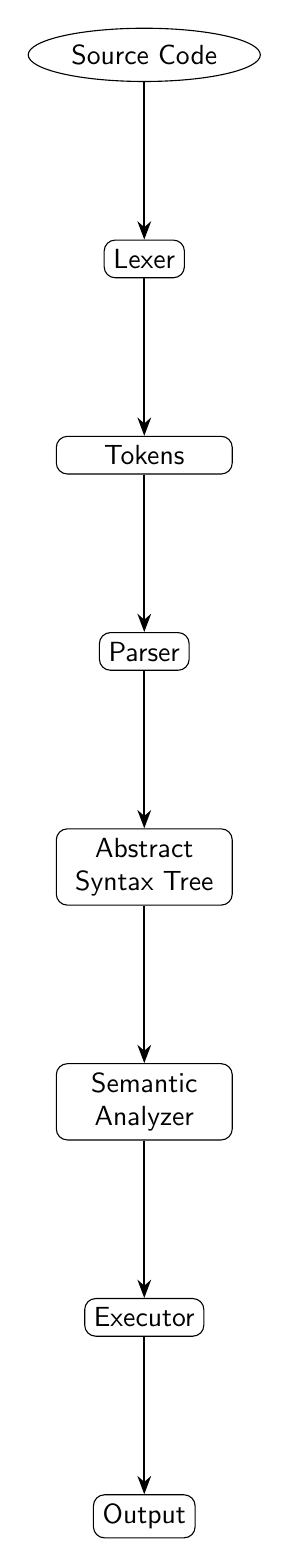
\begin{tikzpicture}[
  node distance=2cm, 
  every node/.style={rectangle, draw=black, rounded corners, align=center, font=\sffamily},
  arrow/.style={-Stealth, thick}
]

\node (source) [ellipse, draw] {Source Code};
\node (lexer) [below=of source] {Lexer};
\node (tokens) [below=of lexer, text width=2cm] {Tokens};
\node (parser) [below=of tokens] {Parser};
\node (ast) [below=of parser, text width=2cm] {Abstract Syntax Tree};
\node (semantic) [below=of ast, text width=2cm] {Semantic Analyzer};
\node (executor) [below=of semantic] {Executor};
\node (output) [below=of executor] {Output};

\draw[arrow] (source) -- (lexer);
\draw[arrow] (lexer) -- (tokens);
\draw[arrow] (tokens) -- (parser);
\draw[arrow] (parser) -- (ast);
\draw[arrow] (ast) -- (semantic);
\draw[arrow] (semantic) -- (executor);
\draw[arrow] (executor) -- (output);

\end{tikzpicture}

\end{center}

\end{document}
